% Flowchart Task B - multi-agent system with a supervising agent (exam guide 4.2, 7.1)
% Compile: pdflatex task_b_multi_agent.tex
\documentclass[border=10pt]{standalone}
\usepackage[T1]{fontenc}
\usepackage{lmodern}
\usepackage{tikz}
\usetikzlibrary{shapes.geometric, arrows.meta, positioning, fit, backgrounds, calc}

\tikzset{
  base/.style={draw, thick, align=center, font=\small, minimum height=9mm},
  io/.style={base, ellipse, fill=gray!15},
  proc/.style={base, rectangle, rounded corners=2pt, fill=blue!8, text width=76mm},
  llm/.style={base, rectangle, rounded corners=2pt, fill=orange!15, text width=76mm},
  dec/.style={base, diamond, aspect=2.6, fill=yellow!20, inner sep=1pt, text width=32mm},
  agent/.style={base, rectangle, rounded corners=2pt, fill=orange!8, font=\scriptsize,
                text width=21mm, minimum height=8mm},
  side/.style={base, rectangle, rounded corners=2pt, fill=red!8, text width=46mm},
  arr/.style={-{Stealth[length=2.5mm]}, thick},
  lbl/.style={font=\footnotesize\itshape},
}

\hyphenpenalty=10000 \exhyphenpenalty=10000  % no hyphenation inside the boxes
\begin{document}
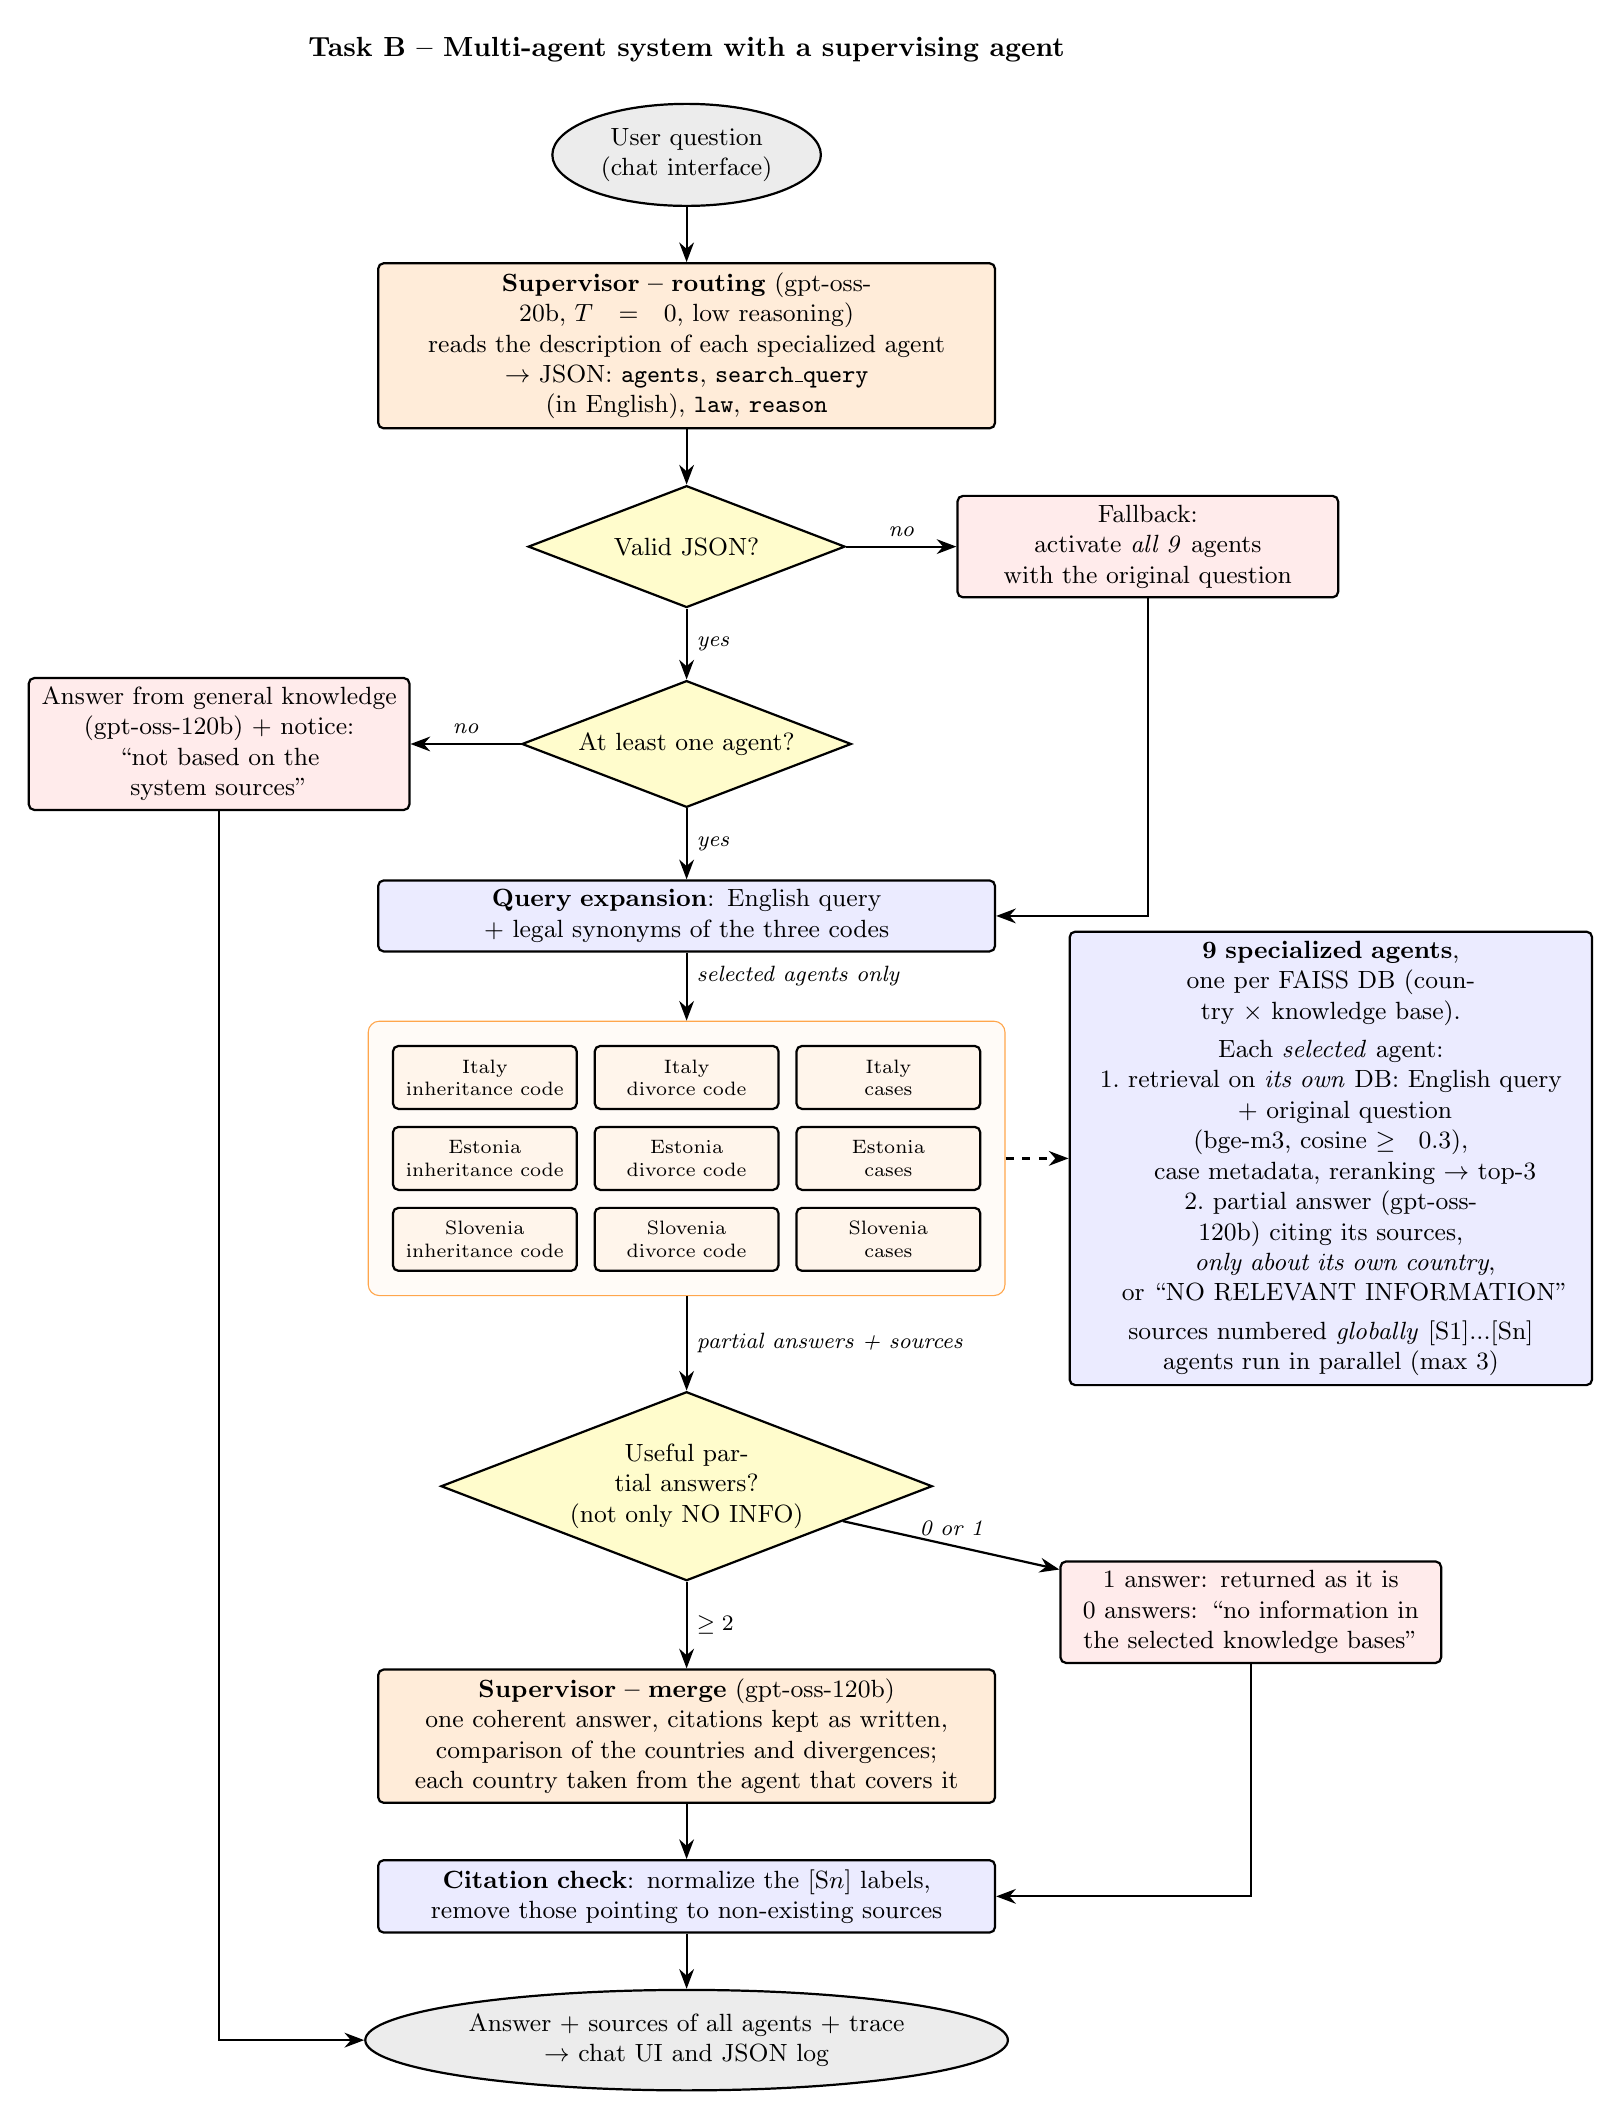
\begin{tikzpicture}[node distance=7mm]

% ---------------- supervisor routing ----------------
\node[io] (q) {User question\\(chat interface)};
\node[llm, below=of q] (sup) {\textbf{Supervisor -- routing} (gpt-oss-20b, $T=0$, low reasoning)\\
  reads the description of each specialized agent\\
  $\rightarrow$ JSON: \texttt{agents}, \texttt{search\_query} (in English), \texttt{law}, \texttt{reason}};
\node[dec, below=of sup] (json) {Valid JSON?};
\node[dec, below=9mm of json] (any) {At least one agent?};
\node[proc, below=9mm of any] (expand) {\textbf{Query expansion}: English query + legal synonyms of the three codes};

% ---------------- the 9 specialized agents ----------------
\node[agent, below=22mm of expand] (a5) {Estonia\\divorce code};
\node[agent, left=2mm of a5] (a4) {Estonia\\inheritance code};
\node[agent, right=2mm of a5] (a6) {Estonia\\cases};
\node[agent, above=2mm of a4] (a1) {Italy\\inheritance code};
\node[agent, above=2mm of a5] (a2) {Italy\\divorce code};
\node[agent, above=2mm of a6] (a3) {Italy\\cases};
\node[agent, below=2mm of a4] (a7) {Slovenia\\inheritance code};
\node[agent, below=2mm of a5] (a8) {Slovenia\\divorce code};
\node[agent, below=2mm of a6] (a9) {Slovenia\\cases};
\begin{scope}[on background layer]
  \node[fit=(a1)(a9), draw=orange!70, rounded corners, inner sep=3mm, fill=orange!3] (agents) {};
\end{scope}

\node[proc, right=8mm of agents, text width=64mm] (work) {\textbf{9 specialized agents},\\
  one per FAISS DB (country $\times$ knowledge base).\\[1mm]Each \emph{selected} agent:\\
  1.\ retrieval on \emph{its own} DB: English query\\
  \phantom{1.\ }+ original question (bge-m3, cosine $\geq 0.3$),\\
  \phantom{1.\ }case metadata, reranking $\rightarrow$ top-3\\
  2.\ partial answer (gpt-oss-120b) citing its sources,\\
  \phantom{2.\ }\emph{only about its own country},\\
  \phantom{2.\ }or ``NO RELEVANT INFORMATION''\\[1mm]
  sources numbered \emph{globally} [S1]...[Sn]\\
  agents run in parallel (max 3)};

% ---------------- merge ----------------
\node[dec, below=12mm of agents] (useful) {Useful partial answers?\\(not only NO INFO)};
\node[llm, below=11mm of useful] (merge) {\textbf{Supervisor -- merge} (gpt-oss-120b)\\
  one coherent answer, citations kept as written,\\
  comparison of the countries and divergences;\\
  each country taken from the agent that covers it};
\node[proc, below=of merge] (check) {\textbf{Citation check}: normalize the [S$n$] labels,\\remove those pointing to non-existing sources};
\node[io, below=of check] (out) {Answer + sources of all agents + trace\\$\rightarrow$ chat UI and JSON log};

% ---------------- side elements ----------------
\node[side, right=14mm of json] (all) {Fallback:\\activate \emph{all 9} agents\\with the original question};
\node[side, left=14mm of any] (nokb) {Answer from general knowledge\\(gpt-oss-120b) + notice:\\
  ``not based on the system sources''};
\node[side, right=16mm of useful, yshift=-16mm] (one) {1 answer: returned as it is\\0 answers: ``no information in\\the selected knowledge bases''};

% ---------------- arrows ----------------
\draw[arr] (q) -- (sup);
\draw[arr] (sup) -- (json);
\draw[arr] (json) -- node[lbl, right] {yes} (any);
\draw[arr] (json) -- node[lbl, above] {no} (all);
\draw[arr] (all) |- (expand);
\draw[arr] (any) -- node[lbl, right] {yes} (expand);
\draw[arr] (any) -- node[lbl, above] {no} (nokb);
\draw[arr] (nokb) |- (out);
\draw[arr] (expand) -- node[lbl, right, pos=0.35] {selected agents only} (agents);
\draw[arr, dashed] (agents) -- (work);
\draw[arr] (agents) -- node[lbl, right] {partial answers + sources} (useful);
\draw[arr] (useful) -- node[lbl, right] {$\geq 2$} (merge);
\draw[arr] (useful) -- node[lbl, above] {0 or 1} (one);
\draw[arr] (one) |- (check);
\draw[arr] (merge) -- (check);
\draw[arr] (check) -- (out);

\node[font=\bfseries, above=4mm of q] {Task B -- Multi-agent system with a supervising agent};
\end{tikzpicture}
\end{document}
